\chapter{\acl{slr}}
\label{chapter:literature-review}

This chapter summarises a \ac{slr} conducted using \ac{prisma} 2020 \cite{Page2021} guidelines\footnote{\url{https://static1.squarespace.com/static/65b880e13b6ca75573dfe217/t/676243b4c4a4752e13bbdfdf/1734493108989/PRISMA_2020_checklist.pdf}} to explore intelligent technologies for improving \ac{lfms}, emphasising advancements in \ac{ai} and \ac{ir}. The review addresses the research's objectives, including evaluating these technologies, identifying implementation challenges, and establishing best practices. This chapter also emphasises the progress in object recognition and multimodal matching and identifies scalability, computational, and ethical challenges, paving the way for future research to enhance \ac{lf} systems.

\section{Research Question and Methods} \label{subsec:slr}

\ac{lf} management has historically presented numerous challenges across both public and private sectors, as underlined in a wealth of academic articles and studies \cite{Prawira2024}. To address previously mentioned persistent issues and uncover effective solutions, a rigorous \ac{slr} was undertaken, focusing specifically on innovations, challenges, and best practices in the realm of intelligent lost property management. The review was designed with a methodological rigour that adheres to the \ac{prisma} 2020 checklist of items, guaranteeing that every aspect of the research was conducted with the highest standards of integrity and transparency. By synthesising the latest uncovered findings, the \ac{slr} offers not only a comprehensive understanding of the current landscape but also valuable insights that can inform the design of a \ac{lfms} system. The \ac{slr} later resulted in the production of a document directly aligned with this dissertation's scope, named \textit{"Designing an Intelligent Solution for Lost Property Management: A Systematic Review"}.

The review sought to answer the central research question \textit{"How can intelligent technologies enhance the efficiency and user experience of lost property management systems?"}, which refers to how \ac{ai}-based technologies such as \ac{cv} and \ac{nlp} and many others can provide solutions to the inefficiencies in \ac{lf} management. The \ac{slr} analysed numerous articles and integrated 18 high-quality studies that demonstrated the capacity to provide new insights into the investigation area. The mentioned research question was then separated into the following three major objectives:

\begin{itemize}
\item Evaluating the applicability of the selected technologies;
\item Examining existing challenges in implementing these technologies;
\item Identifying best practices to inform the design and development of a proposed system.
\end{itemize}

The \ac{slr} employed a comprehensive four-phase approach associated with the selected \ac{prisma} framework. During the identification phase, academic databases such as Scopus and Web of Science were queried using targeted keywords like \ac{lf} Management, \ac{ims}, \ac{ai}, \ac{nlp}, and \ac{llm}, resulting in an initial yield of 476 studies. These were screened for relevance through the removal of duplicates and an abstract examination. In the eligibility phase, full-text articles were meticulously assessed against predefined inclusion criteria, which focused exclusively on studies published between 2020 and 2024 that addressed \ac{ai}-based solutions. Non-peer-reviewed works and studies lacking empirical validation were excluded. Additionally, to ensure the strength of the \ac{slr}, a quality assessment framework evaluated the methodological rigour and relevance of each study. Each study was rated on its technological contributions and practical applicability. Only those scoring consistently high across all criteria were included. Ultimately, in the inclusion phase, 18 studies were selected and categorised based on the technologies employed. This categorisation can be better analysed in Figure \ref{fig:prisma_results}, which includes the distribution of the technologies and frameworks explored and the most signigicant challenges pointed out. Figure \ref{fig:prisma_workflow} illustrates the \ac{prisma} flowchart, summarising the selection process. A thematic analysis was conducted, extracting valuable results into the contributions of each technological domain.

\begin{figure}[!htb]
    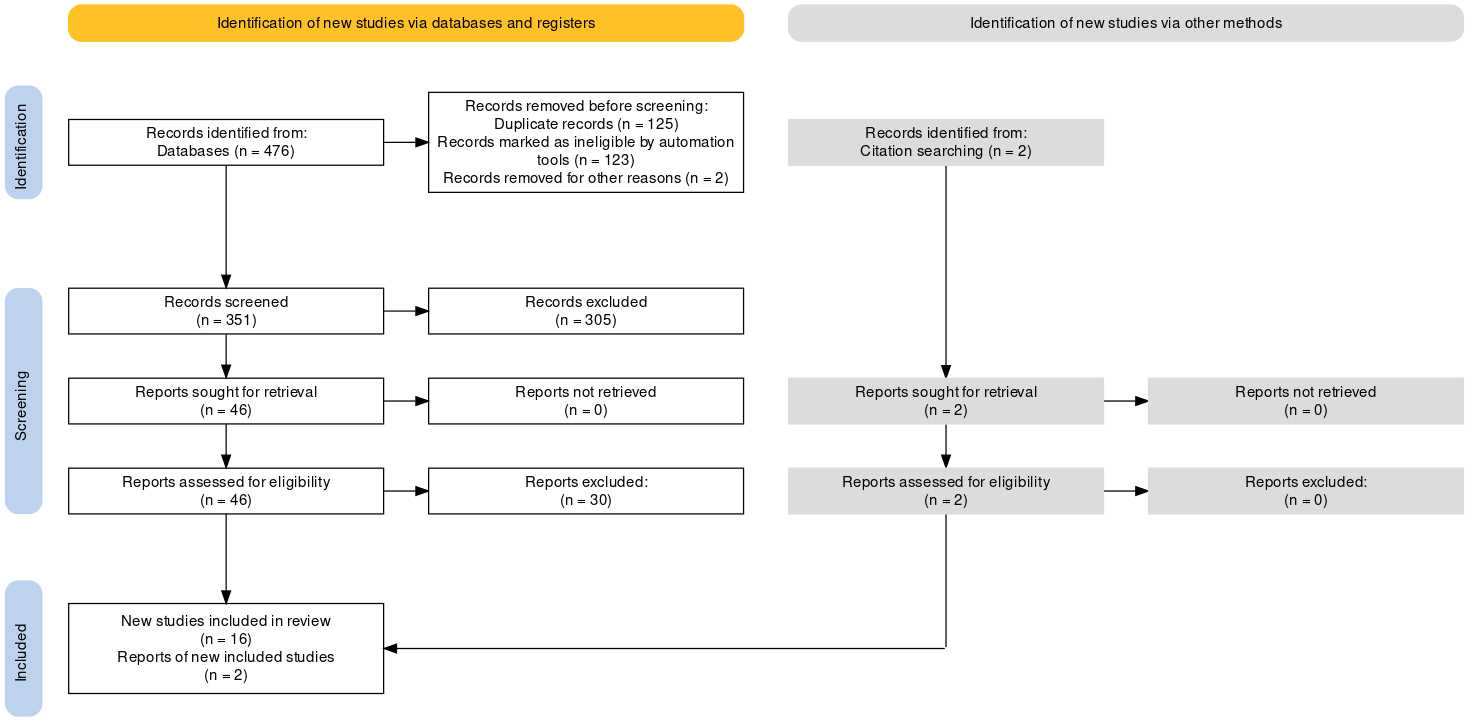
\includegraphics[width=0.95\textwidth]{figs/chapter2/prisma.png}
    \centering
    \caption[\acs{prisma} 2020 flow diagram with a described quantity of research in each step.]{\acs{prisma} 2020 flow diagram with a described quantity of research in each step.}
    \label{fig:prisma_workflow}
\end{figure}

\begin{figure}[!htb]
    \begin{subfigure}{1\linewidth}
        \begin{tikzpicture}
            \pie[sum=auto,rotate=180,text=legend,radius=1.5]{13/\acs{yolo}, 4/\acs{resnet}-50, 1/Traditional Feature-Based Methods, 1/Cosine Similarity, 1/Euclidean Distance}
        \end{tikzpicture}
        \centering
        \caption{Technologies and Frameworks}
    \end{subfigure}

    \vspace{0.5cm}

    \begin{subfigure}{1\linewidth}
        \begin{tikzpicture}
            \pie[sum=auto,text=legend,radius=1.5]{5/Computational Intensity, 5/Dataset Quality Bias, 4/Scalability, 3/Multimodal Integration Complexity, 1/Ethical and Privacy Concerns, 1/Cost of Implementation and Integration}
        \end{tikzpicture}
        \centering
        \caption{Challenges}
    \end{subfigure}
    \centering
    \caption{Distribution of technologies and frameworks explored and mentioned biggest challenges in the selected studies incorporating the \acl{slr}.}
    \label{fig:prisma_results}
\end{figure}

\section{Object Recognition and Categorisation} \label{subsec:object-recognition}

Object recognition and categorisation are processes in the domain of \ac{ai} and \ac{cv}. Object recognition involves identifying objects within an image or video and distinguishing them based on predefined features. Categorisation goes a step further by grouping identified objects into classes and/or groups of classes based on shared attributes or relationships \cite{Liu2021}. These tasks are foundational to numerous applications, including autonomous vehicles, facial recognition, surveillance systems, and many others.

The origins of object recognition can be traced back to the early experiments in pattern recognition during the 1950s and 1960s. Early approaches relied heavily on rule-based systems, where objects were identified using manually defined features such as edges, corners, or textures. \citeauthoryear{Marr1982}'s seminal work on computational vision in the 1980s introduced the concept of multi-level processing, exposing the importance of integrating both low-level (e.g., edge detection) and high-level (e.g., semantic) features. The field evolved significantly in the 1990s with the advent of statistical methods and \ac{ml}. Techniques like support vector machines and decision trees provided more robust frameworks for categorisation \cite{Bishop2006}. Concurrently, datasets such as MNIST\footnote{\url{https://yann.lecun.com/exdb/mnist/}} and ImageNet\footnote{\url{https://www.image-net.org/}} emerged, enabling standardised benchmarking and driving advancements in recognition accuracy.

The evolution of object recognition and categorisation has been marked by the rise of \ac{dl} in the 2010s. \acp{cnn}, such as AlexNet\footnote{\ac{cnn} architecture, designed by Alex Krizhevsky in collaboration with Ilya Sutskever and Geoffrey Hinton at the University of Toronto in 2012} and \ac{resnet}, models capable of leveraging feature extraction, revolutionised this field by achieving human-like performance on challenging tasks. These models finally enabled the recognition of complex patterns and relationships in data \cites{He2015, Krizhevsky2017}. More recently, transformer-based architectures, exemplified by vision transformers, have further enhanced the capabilities of recognition systems. These models utilise attention mechanisms to capture long-range dependencies and contextual information, surpassing the limitations of traditional \acp{cnn} \cite{Dosovitskiy2020}.

\acp{cnn}, particularly \ac{resnet}-50, are widely utilised due to their remarkable capability to extract visual features. Studies have shown that ResNet-50 achieves high accuracy in identifying objects with varying attributes and appearances, a critical aspect for handling the heterogeneity of \ac{lf} items such as electronics, accessories, or apparel \cites{Prawira2024, Ghazal2016, Liu2022}. Similarly, \ac{yolo} models, including \ac{yolo}v7, are renowned for their real-time detection capabilities, ensuring low-latency processing and high precision even in challenging environments such as low light or cluttered backgrounds \cites{Sharma2024, Vedanth2024}.

\ac{resnet}-50, short for \acl{resnet} with 50 layers, has a \ac{dl} architecture designed to address the vanishing gradient problem in very deep neural networks. It introduces shortcut connections, or residual blocks, that allow gradients to flow more effectively during backpropagation, securing better convergence during training. \ac{resnet}-50 has become a standard in computer vision tasks due to its balance of depth and computational efficiency, making it suitable for extracting intricate visual features from diverse datasets \cite{He2015}. Its ability to generalise across object categories makes it a reliable choice for \ac{lf} management applications. \ac{yolo} is an object detection algorithm known for its speed and accuracy. Unlike traditional methods that scan an image region by region, \ac{yolo} processes the entire image in a single pass, predicting bounding boxes and class probabilities simultaneously, which significantly reduces computation time while maintaining high detection precision. \ac{yolo}v7, a more recent iteration, builds on these strengths by introducing architectural improvements for better performance in real-time scenarios, including high-density environments like traffic monitoring \cites{Redmon2015, Wang2022}.

Object recognition models can struggle with computational intensity, requiring significant resources for training and deployment \cites{Lubna2021, Mezhenin2021}. Lightweight versions of models are being developed to mitigate these issues, particularly for mobile applications, which are essential for systems designed to be universally accessible. Mobile-compatible frameworks, using optimised \ac{cnn}, provide the added advantage of enabling real-time item reporting and retrieval through user-friendly interfaces, expanding the reach of such systems \cites{Stout2024, Ghazal2016}.

Furthermore, these systems still need to contend with the diverse characteristics of objects. Items with subtle features or ambiguous shapes often pose difficulties for detection algorithms. Addressing this requires extensive and diverse datasets for training and validating in order to ensure that models can generalise effectively without overfitting to specific item categories \cites{Prawira2024, Liu2022, Sharma2024}. Hybrid approaches that integrate multiple algorithms or modalities are emerging as strategies to overcome these limitations. For instance, combining cloud-based data synchronisation with multimodal recognition has improved retrieval rates by facilitating large-scale processing and analysis \cite{Liu2024, Vedanth2024}.

\section{\acl{nlp}} \label{subsec:nlp}

\ac{nlp} is a multidisciplinary field at the intersection of linguistics, computer science, and artificial intelligence, enabling machines to process, understand, and generate human language. \ac{nlp} encompasses two core subfields: \ac{nlu} and \ac{nlg} \cite{Khurana2023}. \ac{nlu} focuses on interpreting and extracting meaning from textual or spoken language, including tasks such as sentiment analysis, intent recognition, and entity extraction, allowing systems to comprehend user input and respond accordingly \cite{Khurana2023}. In contrast, \ac{nlg} involves creating coherent and contextually appropriate textual or spoken output from structured data, such as generating summaries, reports, or conversational responses \cite{Dong2021}.

The origins of \ac{nlp} date back to the 1950s, when \citeauthoryear{Turing1950} proposed the concept of machine intelligence in his seminal work "Computing Machinery and Intelligence". One of the early milestones was the development of the Georgetown-IBM experiment in 1954, which demonstrated automatic translation between Russian and English, albeit limited to a small vocabulary and specific grammatical constructs. This marked the beginning of using computers to process and understand human language \cite{Hutchins2004}. About 50 years later, in the 1990s and early 2000s, \ac{ml} algorithms, mainly supervised learning, began to dominate \ac{nlp}, enhancing part-of-speech tagging, named entity recognition, and sentiment analysis. This era also witnessed the rise of the first large-scale resources for \ac{nlp}, including the Penn Treebank\footnote{https://catalog.ldc.upenn.edu/docs/LDC95T7/cl93.html} and WordNet\footnote{https://wordnet.princeton.edu/}, which provided valuable training data and lexical knowledge \cite{Marcus1993, Fellbaum1998}.

More recently, the new era has been characterised by a revolution in \ac{nlp} fueled by \ac{dl}. Neural network architectures, particularly recurrent neural networks and their derivatives, long short-term memory networks, demonstrated remarkable capabilities in sequence-to-sequence tasks such as translation and text summarisation \cite{Bahdanau2015}. Furthermore, the introduction of attention mechanisms and transformer-based models, such as \ac{bert} and \ac{gpt}, has drastically improved the state of the art, enabling unprecedented performance across a wide range of \ac{nlp} tasks \cite{Vaswani2017, Devlin2019}. Today, \ac{nlp} continues to evolve, integrating cutting-edge advancements in \ac{ai}, including transfer learning and pre-trained language models, to achieve higher accuracy and efficiency in a variety of complex tasks, namely sentiment analysis, machine translation, and conversational agents \cite{Howard2018}.

The systematic review highlights the growing role of \ac{nlp} in intelligent systems, particularly in enhancing human-computer interaction and automating complex processes. For instance, \ac{nlu} is central to enabling systems to interpret user input, extracting key entities, sentiments, and intents. \citeauthoryear{Prawira2024} and \citeauthoryear{Ghazal2016}, have already adopted these capabilities in their \ac{lfms} to streamline the reporting and retrieval of lost items. By leveraging \ac{nlu} models, their systems can process user descriptions into structured data that, once properly stored and indexed, can later be matched against found items.

Despite these advancements, several challenges remain. Scalability and computational efficiency are ongoing concerns, particularly when deploying \ac{nlp} models in real-time applications. Additionally, ethical considerations, including bias in language models and data privacy, require attention to ensure the responsible use of \ac{nlp} technologies \cite{Prawira2024}.


\section{Multimodal Matching} \label{subsec:multimodal-matching}

Embeddings play a pivotal role in modern artificial intelligence, particularly for applications requiring the integration of multimodal data such as images and text. These embeddings transform high-dimensional data into a lower-dimensional vector space while preserving semantic relationships. For example, image embeddings are often generated using \ac{cnn}, whereas text embeddings leverage transformer-based models \cite{He2015, Devlin2019}. This dimensionality reduction enables efficient and meaningful comparisons across large datasets.

Similarity search is a cornerstone technique in embedding-based systems. \citeauthoryear{Prawira2024} and \citeauthoryear{Ghazal2016} have experimented with metrics such as cosine similarity and Euclidean distance in order to quantify the proximity between embeddings, offering probabilistic measures of match likelihood between simulated \ac{lf} items. A high cosine similarity score, for instance, suggests strong alignment between query and database entries. Probabilistic models can further refine these measures, incorporating confidence intervals that guide the decision-making \cite{Dosovitskiy2020}.

Considering the domain of \ac{lf} management, embeddings would facilitate the matching of user-provided data to stored items or records. Visual embeddings derived from processed, uploaded images would be compared against a database of known items. Similarly, textual embeddings generated from user descriptions and interactions could be matched to metadata or textual entries in the database. When combined, these approaches improve the accuracy of the matching process \cite{Prawira2024, Radford2021}. For instance, the integration of image and text embeddings through models like \ac{clip} enables effective multimodal matching by aligning visual and textual information in a unified vector space \cite{Radford2021}.

On the one hand, embedding-based systems face challenges related to scalability, bias, and computational demands. Scaling these systems to handle large datasets requires optimisation techniques such as lightweight models or distributed computing \cite{Lubna2021}. Moreover, biases inherent in pre-trained models can affect fairness, mainly when embeddings are derived from imbalanced datasets \cite{Prawira2024}. On the other hand, despite these challenges, empirical studies underscore the efficacy of multimodal matching in \acp{lfms}. For instance, \citeauthoryear{Prawira2024} achieved a 97.92\% matching accuracy by integrating \ac{resnet} embeddings with cosine similarity. \citeauthoryear{Ghazal2016} demonstrated an 89.2\% retrieval accuracy using a multi-feature image matching approach that incorporated texture, shape, and colour features.

% \section{Privacy and Security} \label{subsec:privacy-security}

% Todo: Write this section.

% \section{User Experience} \label{subsec:user-experience}

% Todo: Write this section.

% \section{Gamification} \label{subsec:gamification}

% Todo: Write this section.